\documentclass{tufte-handout}
\usepackage{graphicx}
\usepackage{booktabs}
\usepackage{hyperref}

\title{README on the contents of this folder}
\author{Paul Borrill, Sahas Mulamala}

% THIS IS AN AD-HOC FILE TO Get the 


\begin{document}

\maketitle

%\section{README NOTE ON THE CONTENTS OF THIS FOLDER}

\section{"figures" in Folder "Atomic-Ethernet/Æ-Specifications-ETH}

\subsection{There are no figures (yet) in this folder.    All references should be in the {../Figures} folder one directory above this.}

	{../Figures}
	
There is also a top level FIGURES folder in iCloud Drive.  Ideally we access this from a TOP DOWN absolute path, but MacOS currently has a space in the path name to prevent this:

	/Users/paulborrill/Library/Mobile Documents/com~apple~CloudDocs/FIGURES
	
	We can try modifying this:
	
		/Users/paulborrill/Library/Mobile\~Documents/com~apple~CloudDocs/FIGURES	NOT YET TRIED -- NOT NEEDED (SEE BELOW for Pathname with space in it)
		
		
We could possibly also access the folder with a relative path:

	{../../FIGURES}



\subsection{Testing from the Relative (2 directories up Figures Folder [THIS WORKS]}

\begin{figure}[h]
\centering
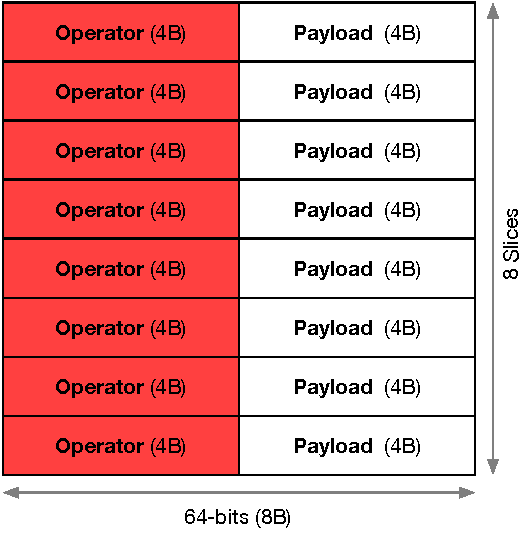
\includegraphics[width=\linewidth]{../../Figures/8-slices.pdf}
\caption{Flow Transactions in Atomic Ethernet -- 8 independent transactions in one SACK-Acknowledged Frame}
\label{fig:Mathematica}
\end{figure}
	
\subsection{Testing from the FIGURES Folder [THIS WORKS]}




\begin{figure}[h]
\centering
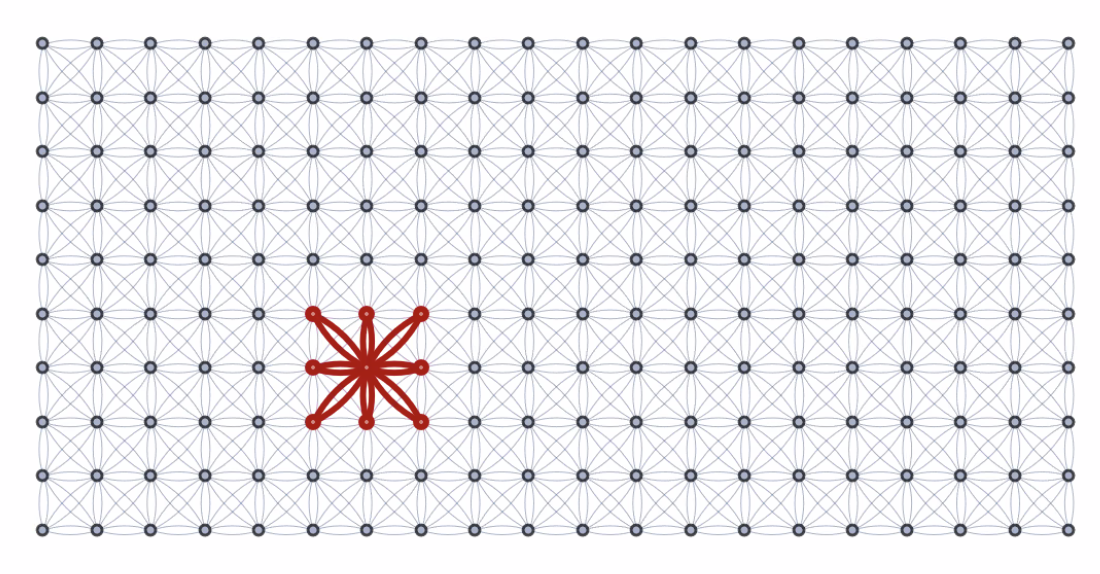
\includegraphics[width=\linewidth]{../../../FIGURES/Mathematica-Tile-png.png}
\caption{Chiplet GROUNDPLANE Abstract Physical Space (lowest layer in  CHIPLET Æthernet) }
\label{fig:Mathematica}
\end{figure}




%\subsection{Lets try this again: Topdown from the FIGURES Folder [THIS WORKS]}
\clearpage
\section{Inspired by Ken Birman's Vortex}

\sidenote{\href{https://www.youtube.com/watch?v=pUla9eyH5uQ}{Vortex Video}}


\begin{figure}[t!]
\centering
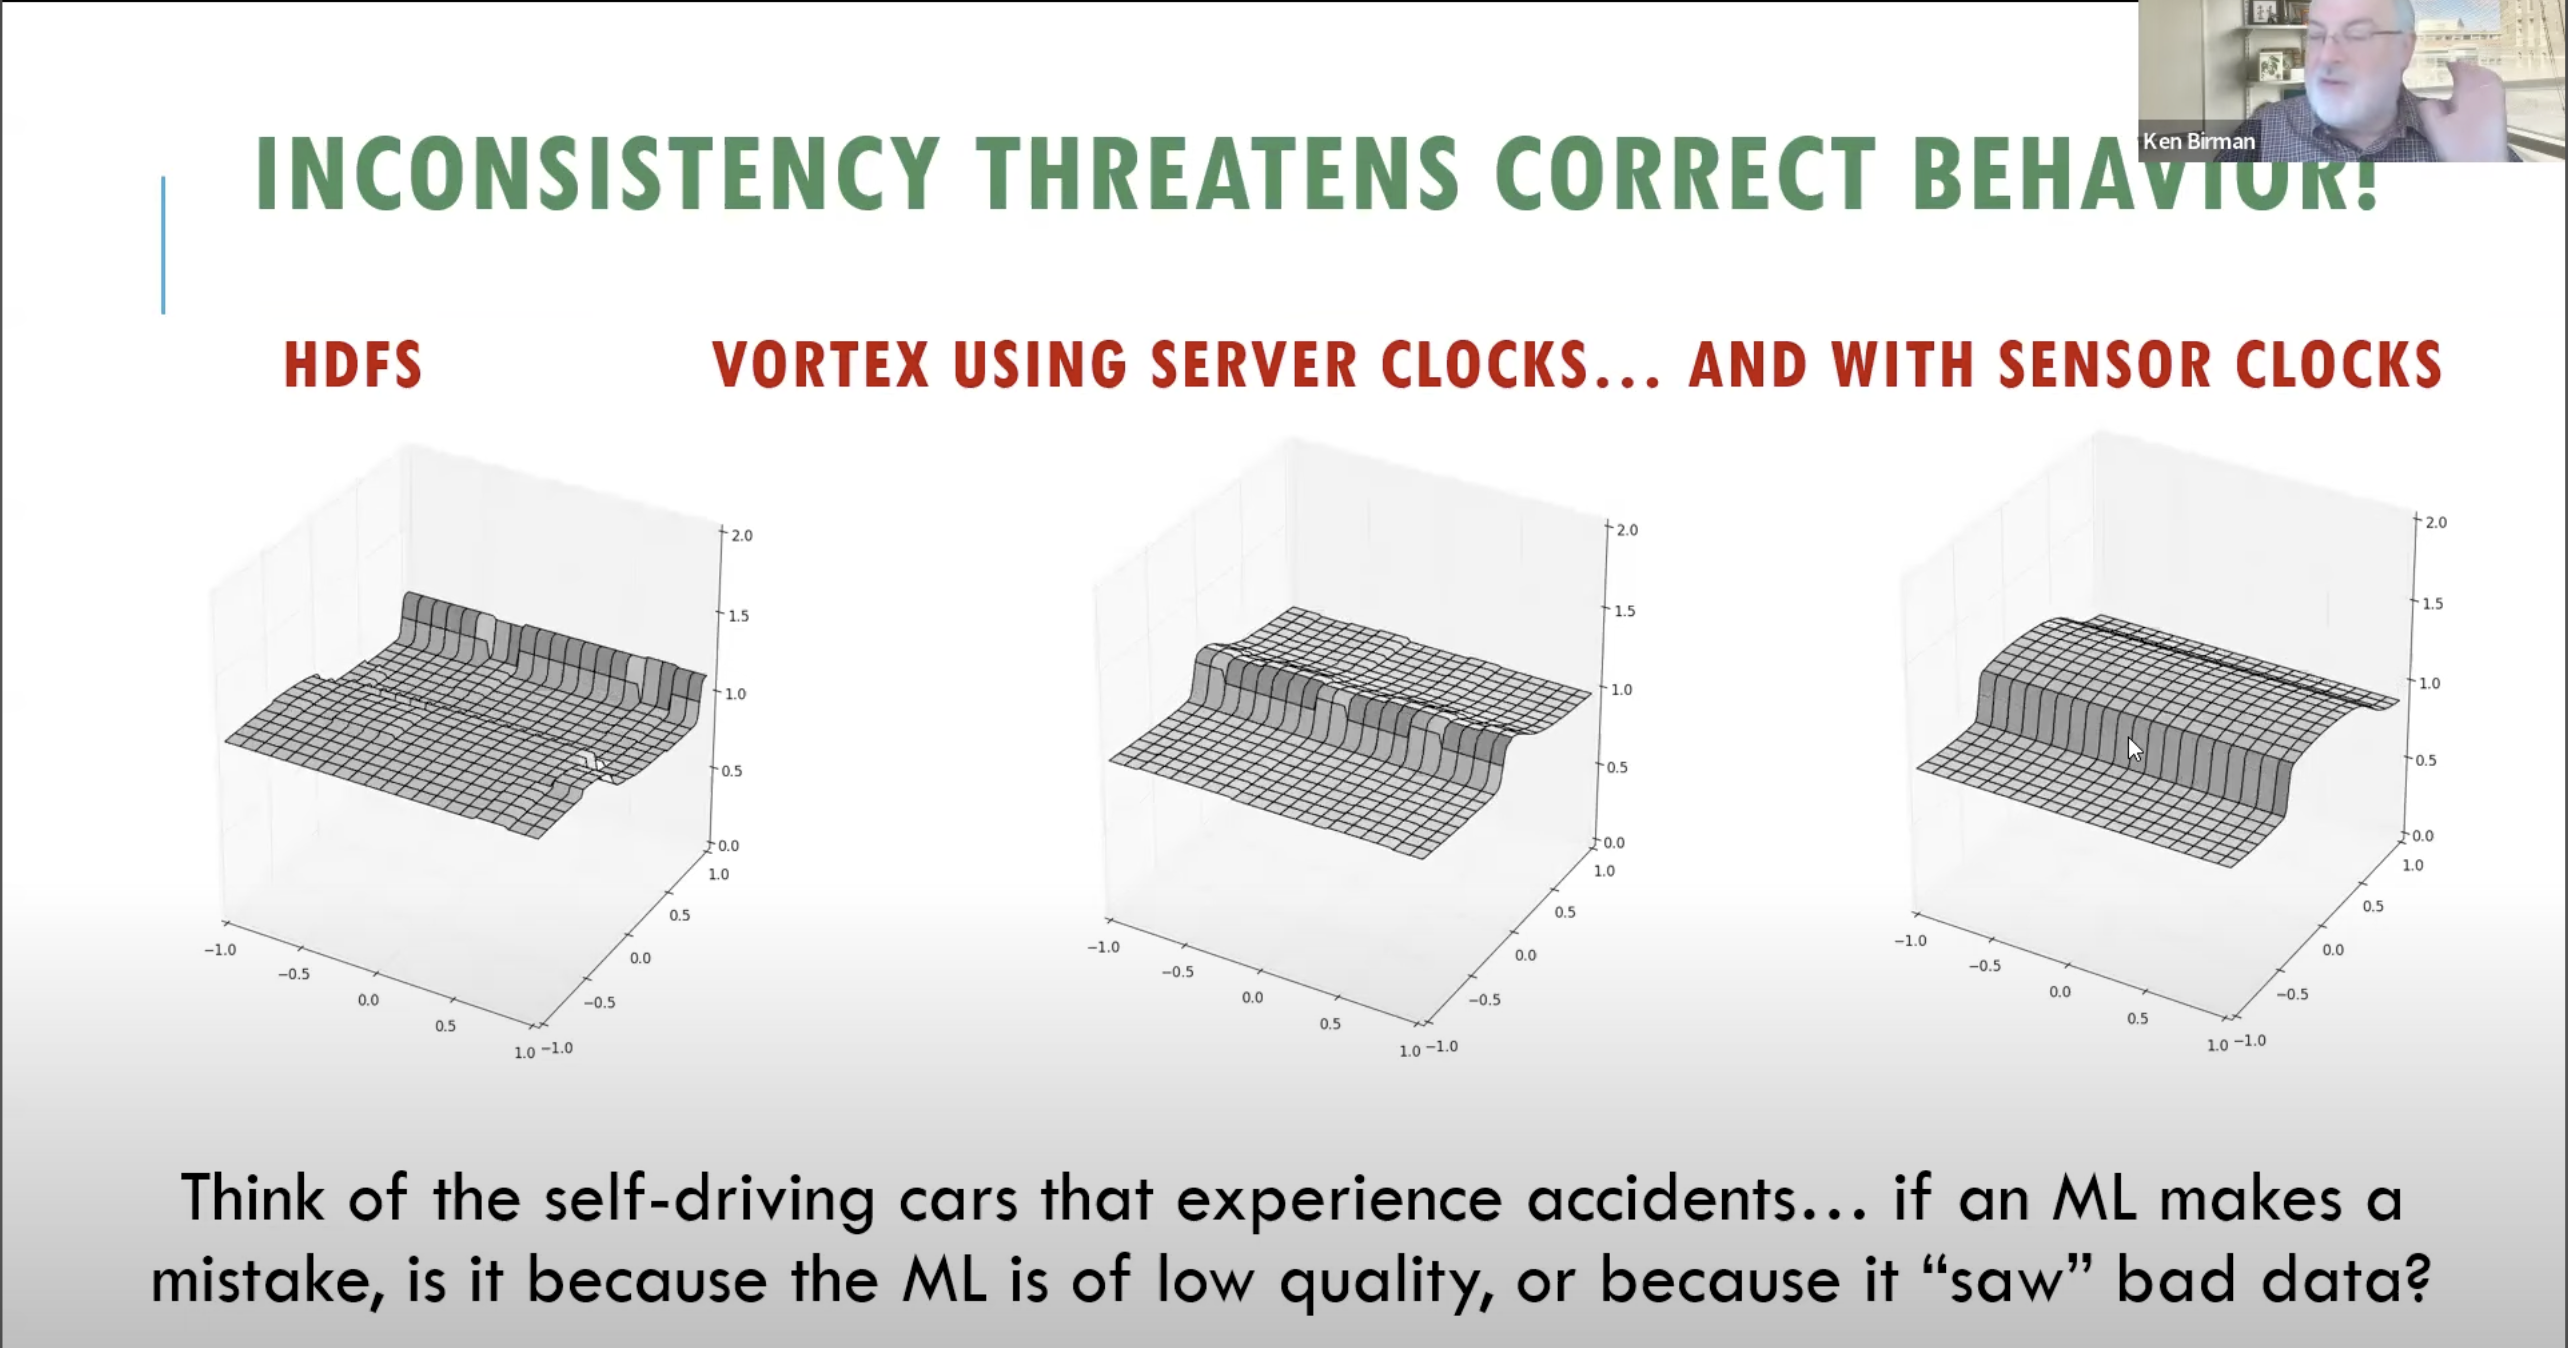
\includegraphics[width=\linewidth]{../../Figures/Vortex.png}
\caption{Ken Birman's Vortex }
\label{fig:Vortex}
\end{figure}


	
\begin{figure}[h!]
\centering
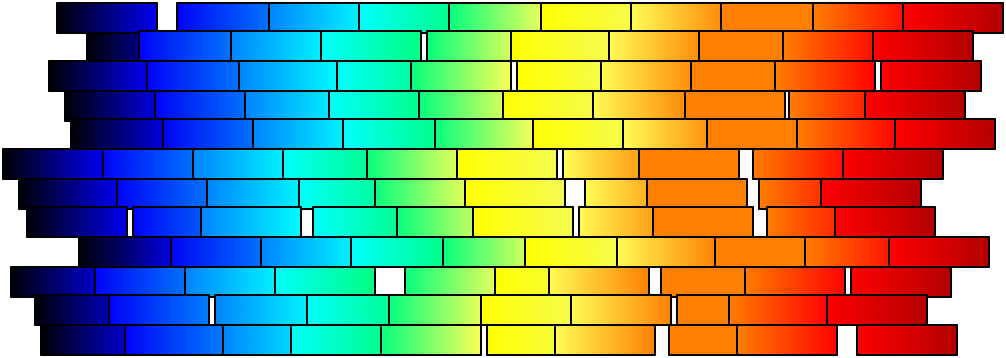
\includegraphics[width=\linewidth]{ /Users/paulborrill/Library/Mobile Documents/com~apple~CloudDocs/FIGURES/Broken-River.png} % This works even though it has a space in the pathname!
\caption{Synchronization Flow without Atomic Ethernet}
\label{fig:Broken-River}
\end{figure}


\begin{figure}[h!]
\centering
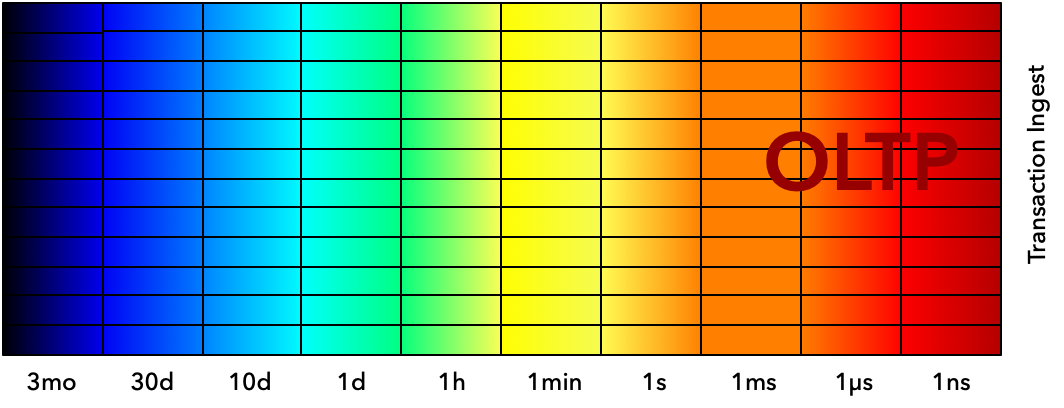
\includegraphics[width=\linewidth]{ /Users/paulborrill/Library/Mobile Documents/com~apple~CloudDocs/FIGURES/River.png} % This works even though it has a space in the pathname!
\caption{Synchronization Flow with Æthernet. Imagine row of Racks (10 Rows each with 12 servers). OR a Chiplet motherboard populated with 120 SmartNICs / IPUs}
\label{fig:River}
\end{figure}



%\begin{figure}[h!]
%\centering
%\includegraphics[width=\linewidth]{ /Users/paulborrill/Library/Mobile Documents/com~apple~CloudDocs/FIGURES/Fat-Tree-for-Time.png} % This works even though it has a space in the pathname!
%\caption{Synchronization Flow with Æthernet. Imagine row of Racks (10 Rows each with 12 servers). OR a Chiplet motherboard populated with 120 SmartNICs / IPUs}
%\label{fig:FatTree}
%\end{figure}

\begin{figure}[h]
\centering
\includegraphics[width=\linewidth]{../../Figures/Fat-Tree-for-Time.png}
\caption{Fat Tree for Time distribution}
\label{fig:FatTree}
\end{figure}
	



\end{document}